\section{Implementation}
\subsection{Matlab}
The first step was to understand the working principle of a DC motor. After getting such knowledge, I had to verify it in Matlab and Simulink. I created two models of a DC motor in Simulink: one built of only basic blocks and second using blocks from the Simscape library. Models are shown on figures \ref{fig:basic} and \ref{fig:hbridge}.

\begin{figure}%[H]
 \begin{center} 
  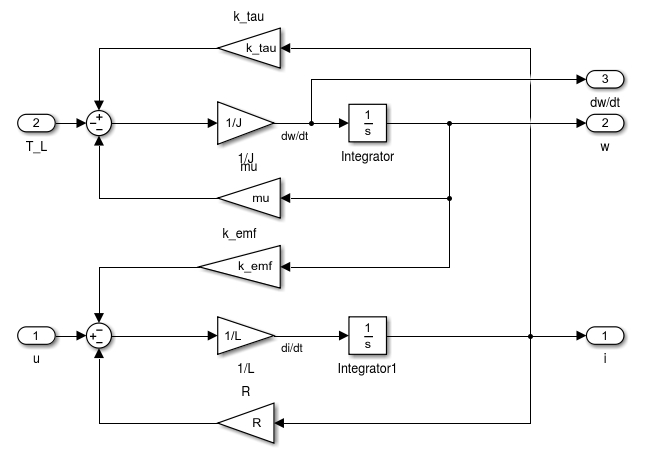
\includegraphics[width=0.7\textwidth]{./stuff/basic_blocks}
 \end{center}
 \caption{A model of a DC motor in Simulink built of basic blocks}
 \label{fig:basic} 
\end{figure}   

\begin{figure}%[H]
 \begin{center} 
  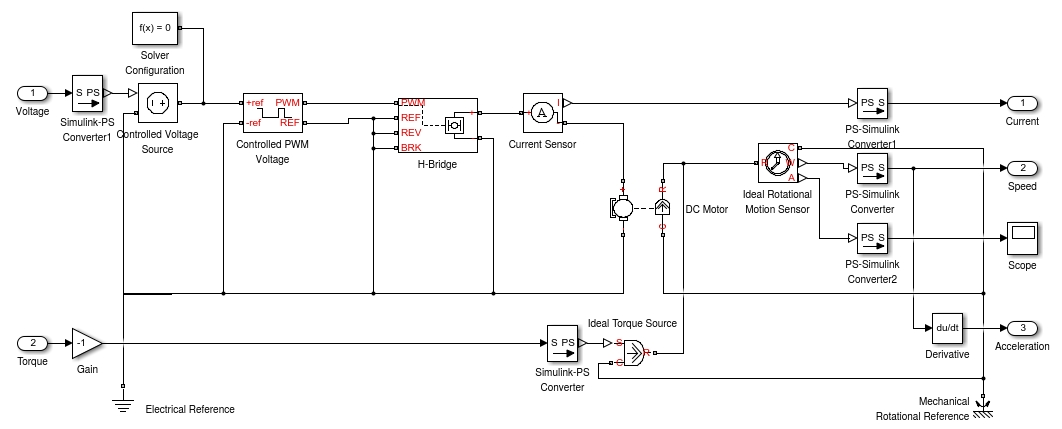
\includegraphics[width=\textwidth]{./stuff/simscape}
 \end{center}
 \caption{A model of a DC Motor in Simulink built of blocks from the Simscape library}
 \label{fig:hbridge} 
\end{figure}   

I tested both models using scripts written in Matlab. Inputs of the system were voltage and applied force, and outputs were current, angular velocity and acceleration. Tests were done for open and closed loop. Control of the process variable was done with a PID controller. Results for both models were almost identical and the simulations confirmed theoretical knowledge and developed my intuition.

\begin{figure}%[H]
 \begin{center} 
  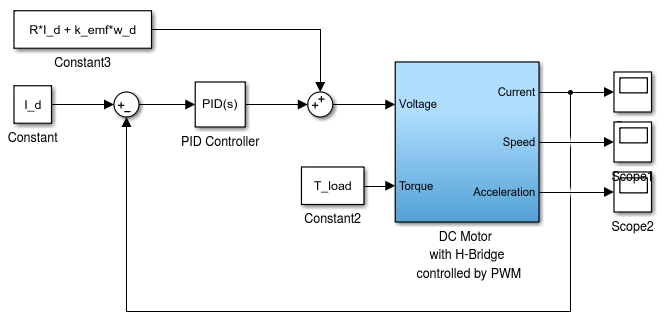
\includegraphics[width=0.7\textwidth]{./stuff/control_loop}
 \end{center}
 \caption{An example control loop with feedforward term}
 \label{fig:loop} 
\end{figure} 

\subsection{Arduino}
Afer getting some experience, I started working with hardware. The computations and control were done by \textsf{Arduino Due} board. The code was written in \textsf{C++}. With such combination, I was able to write a program containing a lot of operations using a high-level programming language.

Control of speed and direction of the motor's movement was done with use of an external H-Bridge and a PWM signal from \textsf{Arduino}.

Arduino was connected with a computer through a serial port. As a middleware \textsf{The Robot Operating System} was used. \textsf{ROS} allowed to change parameters on-line and provided opportunity to observe and visualize values of chosen variables.

Thanks to usage of encoders and measuring the current flowing through the motor, I was able to implement various types of control, for instance:
\begin{itemize}
	\item current (force) control,
	\item position control,
	\item velocity control,
	\item stiffness control,
	\item impedance control,
	\item parallel force/position control.
\end{itemize}  

Because the control was dedicated for a gripper, the most important was the first one.

\subsection{Documentation}
All files with a detailed documentation of the code generated by \textsf{Doxygen} are available at the \textsf{GitHub} repository.